%%% CogSci 2027 six-page paper draft (behavior-first adaptation).
%%% Format target: 6 pages including figures, tables, and any appendix; references may
%%% extend beyond page 6. Template: cogsci.sty from the official 2026 template repository
%%% (github.com/neilbramley/cogscisoc); replace with the 2027 template when posted.

\documentclass[10pt,letterpaper]{article}

\usepackage{cogsci}
% \cogscifinalcopy %%% Uncomment only for the camera-ready version

\usepackage[
  style=apa,
  natbib=true,
  annotation=false,
]{biblatex}
\addbibresource{references.bib}
\setlength{\bibhang}{.125in}

\usepackage{float}
\usepackage{graphicx}
\usepackage{booktabs}
\usepackage{amsmath}

\newcommand{\contrast}{C_{\mathrm{att-acc}}}
\newcommand{\intentbeta}{\beta_{\mathrm{intent}}}
\newcommand{\outcomebeta}{\beta_{\mathrm{outcome}}}

\title{Passing False-Belief Tests Is Not Using Intent:\\
Graded Moral Judgment in Language Models}

\author[1]{\mbox{Anonymous}}
\affil[1]{Anonymous}

\begin{document}

\maketitle

\begin{abstract}
Language models increasingly pass explicit false-belief tests, but it is unclear whether they apply mental-state information when it matters downstream.
We adapted a belief $\times$ outcome moral-judgment paradigm to 20 open-weight and nine closed-API models.
Adults condemn failed harmful attempts more than accidental harms; none of the 20 open models reproduced this ordering, and 14 reversed it.
Six open instruct models answered 82--99\% of hard false-belief items correctly while showing this reversal.
Closed models were heterogeneous: four of nine placed attempts above accidents.
Supervised fine-tuning was sufficient to induce the outcome-dominant profile in three public training pipelines, and internal analyses showed that intent was decodable but did not track or steer ratings.
Explicit false-belief success therefore appears insufficient evidence that a model uses intent in graded social judgment.

\textbf{Keywords:}
theory of mind; moral judgment; intent; large language models; false belief; development
\end{abstract}

\section{Introduction}

Theory of mind (ToM) is usually operationalized as representing another agent's beliefs, desires, or intentions.
Language models now perform well on many explicit false-belief and social-reasoning benchmarks \citep{gandhi2023bigtom,kosinski2024evaluating,chen2024tombench,strachan2024testing}, yet theoretically irrelevant alterations and stress tests can sharply reduce apparent competence \citep{ullman2023alterations,shapira2024clever}.
This creates a construct-validity problem.
A correct answer to ``where will Sally look?'' shows that a model can produce the target answer in that context; it does not show that the model will \emph{use} the same information when a downstream judgment depends on it.
Recent benchmarks have begun to separate explicit inference from applied ToM \citep{gu2026simpletom}.

Moral judgment offers a well-characterized test of applied mental-state use.
In the belief $\times$ outcome paradigm \citep{young2007neural,young2008belief,young2009innocent}, an agent holds a benign or harmful belief and produces a benign or harmful outcome, yielding four cells: neutral, accidental harm, attempted harm, and intentional harm.
Adults condemn a failed attempt (bad belief, no harm) much more than an accident (benign belief, harm), indicating strong reliance on belief and intent \citep{young2007neural}.
Children shift from outcome- toward intent-based judgment with age \citep{cushman2013development}, and societies differ in how much intent matters \citep{barrett2016societies,curtin2020kinship}.
The paradigm therefore supplies a quantitative profile, not a pass/fail label, and outcome weighting cannot simply be equated with being ``non-human.''

We ask three questions.
(1) Does explicit false-belief success predict intent-sensitive graded moral judgment?
(2) How stable is the intent--outcome profile across models, prompts, and training stages?
(3) Where do model profiles fall relative to adult, developmental, and cross-cultural human references, interpreted descriptively?

\section{Background}

\subsection{Intent and outcome in human moral judgment}
The belief $\times$ outcome paradigm was developed to isolate how mental state and consequence jointly shape condemnation \citep{young2007neural,young2008belief,young2009innocent}, and intent effects vary by moral domain \citep{young2011ignorance}.
Developmental work shows that the balance between intent- and outcome-based judgment changes across childhood \citep{cushman2013development}.
Cross-cultural studies show that strong intent weighting is not universal: the size of the intent effect differs across small-scale and industrialized societies \citep{barrett2016societies,curtin2020kinship}.
These findings make the paradigm useful for machine evaluation precisely because it yields graded weights that can be compared to a range of human profiles rather than to one correct answer.

\subsection{Evaluating ToM in language models}
Procedurally generated false-belief tests \citep{gandhi2023bigtom}, broad benchmark suites \citep{chen2024tombench}, and direct human--model comparisons \citep{strachan2024testing} report strong but construct-dependent performance.
At the same time, small changes to task wording can reverse success \citep{ullman2023alterations,shapira2024clever}.
SimpleToM showed that models can infer a mental state yet fail to apply it when predicting behavior or judging it \citep{gu2026simpletom}, and MoCa showed that aggregate agreement with human moral and causal judgments can hide different factor weights \citep{nie2023moca}.
Probing studies indicate that belief information is linearly decodable from model activations \citep{zhu2024beliefs}, which raises the question of whether decodable information is actually used.

\begin{table}[t]
\centering
\small
\caption{Design and the adult reference profile \citep{young2007neural}, normalized to $[0,1]$.}
\label{tab:design}
\begin{tabular}{@{}lllr@{}}
\toprule
Cell & Belief/intent & Outcome & Adult mean \\
\midrule
Neutral & benign & benign & 0.033 \\
Accidental & benign & harmful & 0.267 \\
Attempted & harmful & benign & 0.933 \\
Intentional & harmful & harmful & 0.967 \\
\bottomrule
\end{tabular}
\end{table}

\section{Methods}

\subsection{Stimuli}
We assembled 298 vignettes from published appendices \citep{young2008belief,young2009innocent,young2011ignorance}: 48 four-cell scenarios from \citet{young2008belief}, 24 scenario identifiers from \citet{young2009innocent}, and ten intentional/accidental items from \citet{young2011ignorance}.
All 2009 scenarios are reprints of 2008 scenarios; we merged them into shared scenario groups, leaving 53 independent groups for resampling and cross-validation.
An integrity audit found trailing text nearly aligned with the outcome label (a contamination flag predicted outcome at 0.966); after repair it predicted at 0.517, the majority rate, and all affected outputs were regenerated.

\subsection{Models and scoring}
The open-weight roster contained 20 base and instruct models from the Qwen2.5, OLMo-2, Mistral/Zephyr, Gemma-2, and Llama-3.1/Tulu families (largest 14B; ten Qwen2.5 variants).
Open models were scored deterministically as the expected value of the probability distribution over valid rating digits, normalized to $[0,1]$ with higher values meaning greater condemnation.
Nine closed-API models (four OpenAI, three Anthropic, two Google) were rerun with three templates, five samples per item, and temperature 1.
Because scoring, sampling, and prompt sets differ, open and closed estimates are reported side by side but never pooled.

\subsection{Measures}
The headline measure is the attempted-minus-accidental contrast $\contrast=\bar y_{\mathrm{attempted}}-\bar y_{\mathrm{accidental}}$.
Positive values mean that failed attempts are condemned more than accidents.
Because the two cells differ on both factors, we also report all four cell means and fit $y\sim\mathrm{intent}\times\mathrm{outcome}$ with random intercepts for scenario group and story, whose simple effects give $\intentbeta$ and $\outcomebeta$.
Intervals are scenario-group bootstraps.
Two audits test measurement assumptions: contrasts were recomputed under four normalizations of the native 1--3, 1--4, and 1--7 scales (endpoint, per-model min--max, and z-scores or ranks within model $\times$ template $\times$ source), and item-level reliability was estimated as Spearman--Brown-corrected split-half correlations over 1{,}000 random rater splits (templates within a model, or models within the base or instruct class), after removing condition means so that it indexes item differences beyond the $2\times2$ design.
Explicit false belief was measured with the hard BigToM condition \citep{gandhi2023bigtom}; ToMi was excluded because an audit found 82\% of the scored slice was not a ToM item.

\subsection{Internal analyses (open models only)}
For eight OLMo-2 and Qwen2.5 checkpoints, logistic probes predicted intent and outcome from hidden states under leave-scenario-group-out folds, read at the final story token and at the end of the belief clause, against span-matched lexical baselines.
We tested whether decodability predicted behavior at the item level and across model pairs with representational similarity analysis \citep{kriegeskorte2008rsa}, and we intervened on two to three instruct models by adding intent or outcome directions to hidden states (with matched random controls) and by linearly erasing outcome \citep{belrose2023leace}.

\subsection{Human references}
The adult reference uses cell means from \citet{young2007neural} Experiment~1 ($n=10$; 12 scenarios; \autoref{tab:design}), giving $\contrast=+0.666$.
Child references are digitized attempted-minus-accidental contrasts from \citet{cushman2013development}: $+0.240$ (ages 4--5), $+0.500$ (6--7), and $+0.630$ (8+).
Cross-cultural references come from a ten-society dataset \citep{barrett2016societies,curtin2020kinship}.
None of these is item-matched to our stimuli, so all comparisons are descriptive and we do not assign developmental ages to models.

\section{Results}

\begin{figure*}[t]
    \centering
    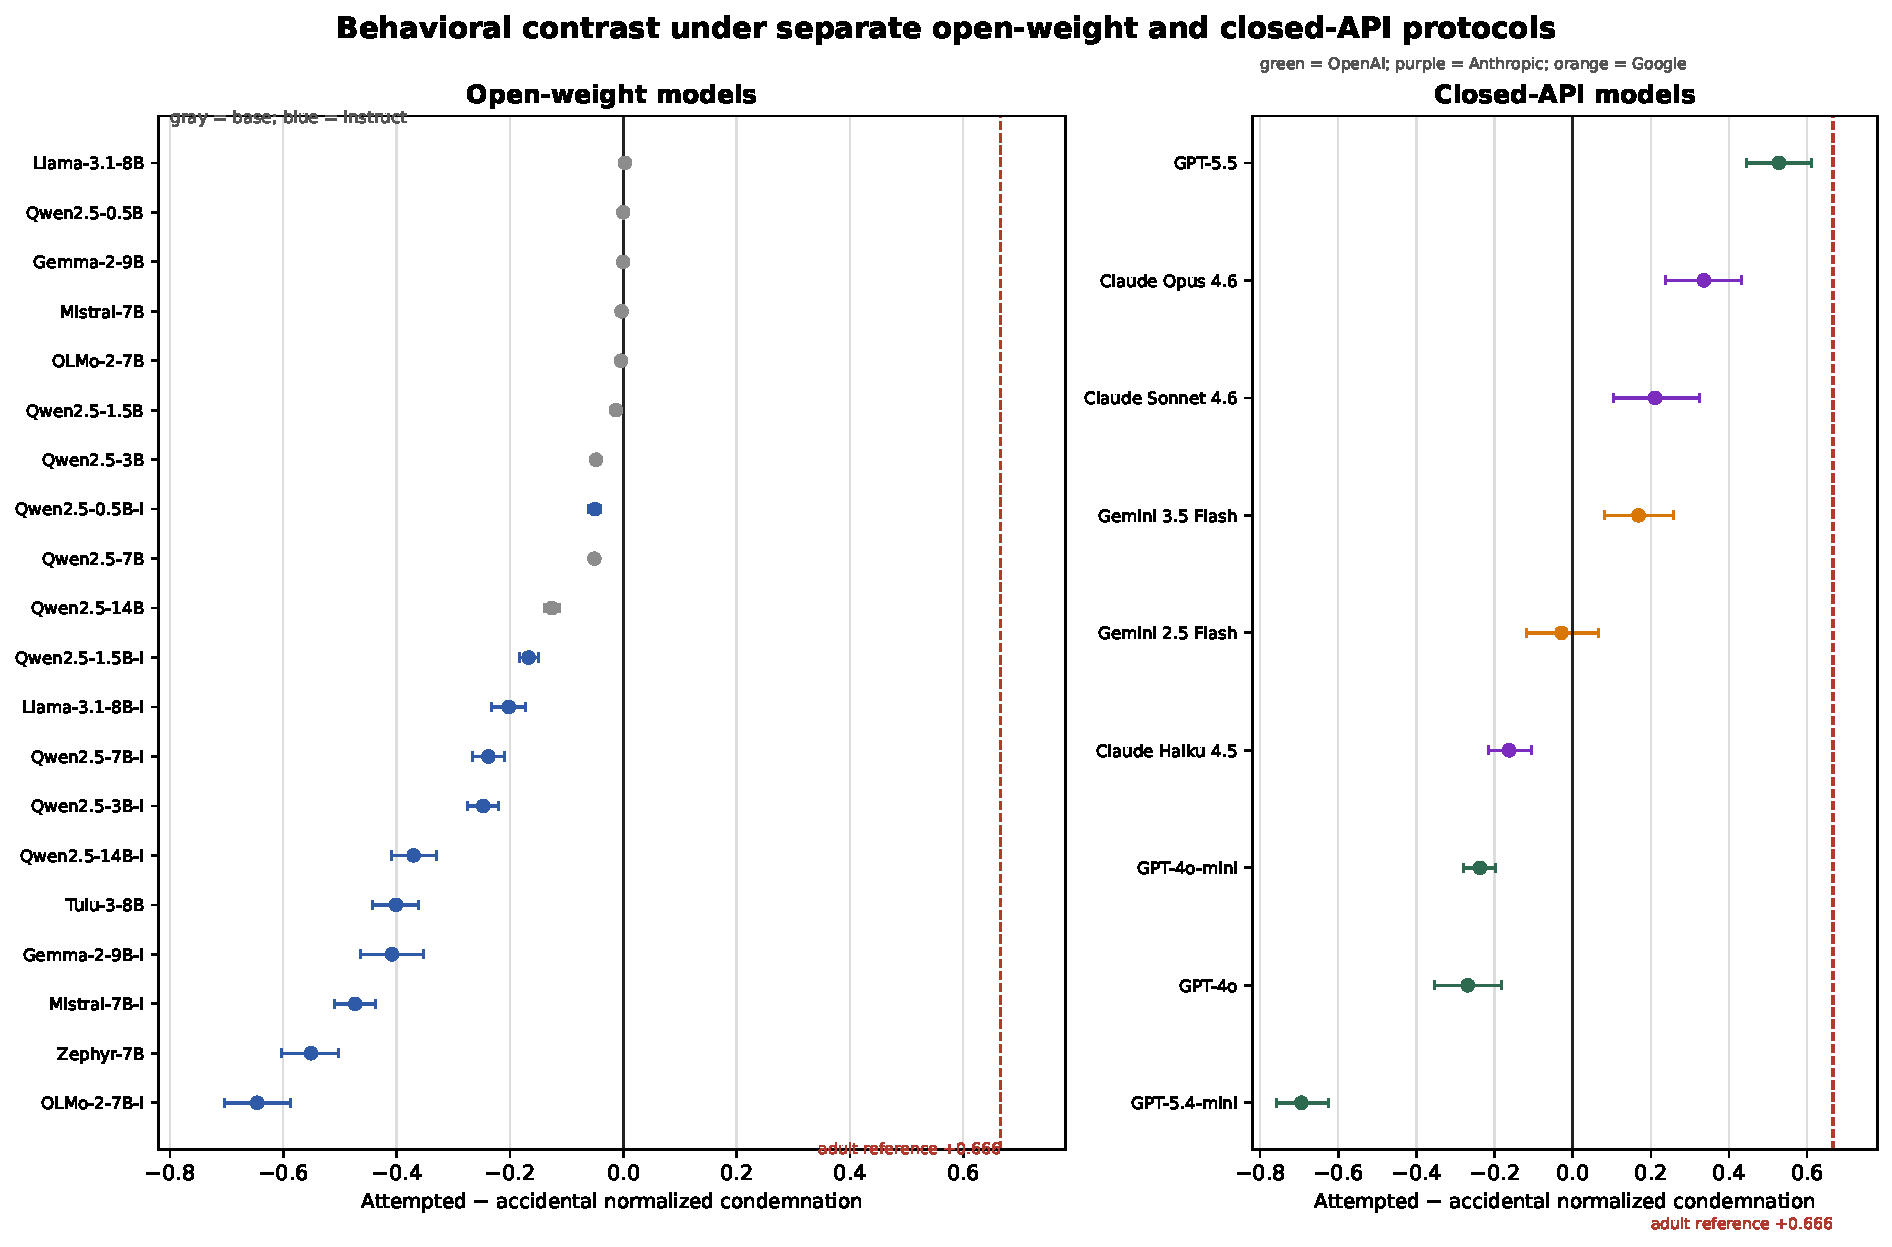
\includegraphics[width=0.92\textwidth]{figures/behavioral_overview.pdf}
    \caption{Attempted-minus-accidental contrast for 20 open-weight models (left; gray = base, blue = instruct) and nine closed-API models (right).
    Positive values place attempted above accidental harm; the dashed line is the non-item-matched adult reference ($+0.666$).
    The two protocols differ in scoring and sampling and are not pooled.}
    \label{fig:overview}
\end{figure*}

\subsection{Open models reverse the adult ordering}
None of the 20 open models reproduced the adult ordering of attempted above accidental harm; 14 reversed it and six were tied (\autoref{fig:overview}).
In the mixed-effects decomposition, 18 of 20 models were outcome-saturating, whereas the adult reference was intent-saturating.
A negative interaction coefficient was not sufficient for human-like resemblance: several models approached the adult interaction magnitude while reversing the underlying attempted/accidental cells.
This illustrates why full cell profiles, not a single interaction term, are needed to compare a model's judgment structure with human data \citep[cf.][]{nie2023moca}.

\subsection{Closed models are heterogeneous}
The closed-API rerun did not support extending this pattern to all current models.
Four of nine models had positive contrasts with intervals excluding zero: GPT-5.5 ($+0.528$ [0.444, 0.610]), Claude Opus~4.6 ($+0.336$ [0.236, 0.432]), Claude Sonnet~4.6 ($+0.211$ [0.104, 0.324]), and Gemini~3.5 Flash ($+0.168$ [0.081, 0.258]).
Four had negative intervals and one interval included zero.
Closed results are behavior-only, and their archival provenance is still being finalized, so we treat them as provisional.

\begin{figure}[t]
    \centering
    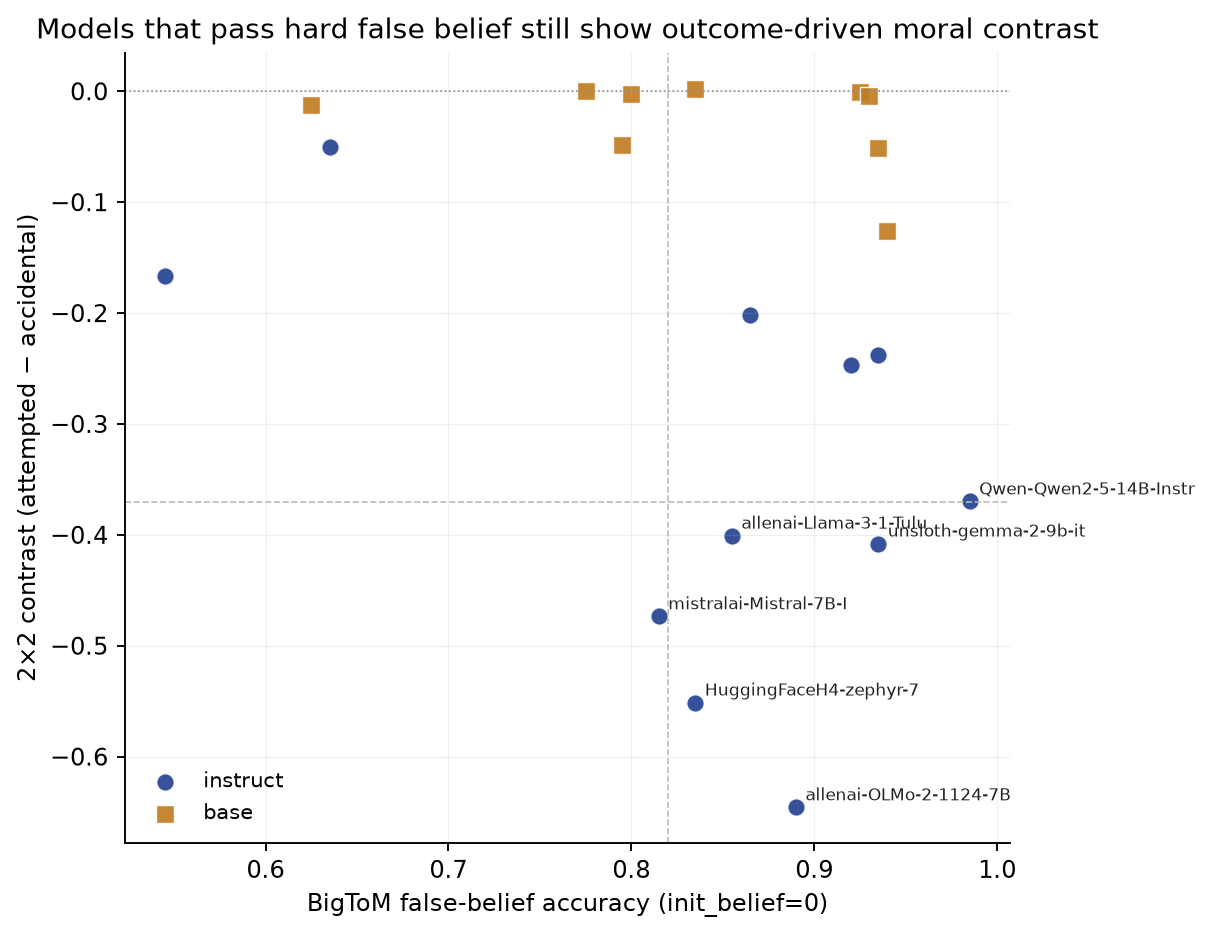
\includegraphics[width=\columnwidth]{figures/tom_vs_contrast.png}
    \caption{Hard false-belief accuracy versus moral contrast for open models.
    Engaged instruct models (blue) pass the false-belief measure while keeping negative contrasts.
    No regression line is interpreted because both axes covary with model type and size.}
    \label{fig:tom}
\end{figure}

\subsection{Explicit false belief does not imply applied intent use}
The six engaged open instruct models scored 0.815--0.985 on hard false-belief items while producing contrasts from $-0.370$ to $-0.646$ (\autoref{fig:tom}).
Every model in this high-false-belief subset therefore fell in the high-explicit, negative-applied quadrant.
This is a within-model coexistence result rather than a correlation; the covariate-adjusted all-model regression was non-significant ($\beta_{\mathrm{ToM}}=-0.379$, $p=0.211$), and instruct-only and within-family intervals were too wide for a directional conclusion (\autoref{tab:bigtom}).

\begin{table}[t]
\centering
\small
\caption{Engaged open instruct models: hard BigToM false-belief accuracy and moral contrast (adult reference $+0.666$).}
\label{tab:bigtom}
\begin{tabular}{@{}lrr@{}}
\toprule
Model & False belief & $\contrast$ \\
\midrule
OLMo-2-7B-Instruct & 0.890 & $-0.646$ \\
Zephyr-7B & 0.835 & $-0.551$ \\
Mistral-7B-Instruct & 0.815 & $-0.473$ \\
Gemma-2-9B-Instruct & 0.935 & $-0.408$ \\
Tulu-3-8B & 0.855 & $-0.401$ \\
Qwen2.5-14B-Instruct & 0.985 & $-0.370$ \\
\bottomrule
\end{tabular}
\end{table}

The dissociation also appeared within the models' own words.
Asked to explain a rating without any cue to mention belief or intent, OLMo-2-7B-Instruct named belief or intent in 81.5\% of stories and Qwen2.5-7B-Instruct in 69.1\%.
Even within those stories, $\outcomebeta/\intentbeta$ was 5.7 and 12.2, and both contrasts remained negative.
Because explanations followed the rating, this shows output-level dissociation, not the cause of the rating.

\subsection{Robustness}
Five of 20 open models changed contrast sign across six common 1--7 prompts, so single-prompt rankings are fragile.
The construct named in the prompt (e.g., wrongness versus punishment) explained approximately 0\% of prompt-factorial variance, and expected-value and sampled scores correlated above 0.95 for 7B instruct models.
Within the five Qwen2.5 base/instruct size pairs, instruction tuning shifted the contrast by approximately $-0.216$ on average ($p\approx0.020$ in the paired test; Wilcoxon $p\approx0.063$).
The separate normalization audit, which covers all nine open base/instruct pairs from five families, found the same direction: the mean instruct-minus-base contrast was $-0.319$ [$-0.345$, $-0.291$] under endpoint scaling, and every pair was negative with an interval excluding zero under endpoint and per-model min--max scaling.
Under within-cell z-scores and ranks the class difference stayed negative but Qwen2.5-14B reversed, so pair estimates are not normalization-invariant, and nine pairs do not establish a universal instruction effect; the model ordering was stable across schemes (Spearman $\rho\geq0.94$ over 34 rater entries).
Item differences beyond the $2\times2$ design were reproducible across instruct models (within-condition split-half 0.83--0.93 across the three sources) but less so across base models (0.36--0.64), and items clustered by outcome (adjusted Rand index 0.88) rather than by intent or source.
A six-model prompt curriculum (belief cues, worked examples, few-shot examples, an explicit intent principle) met its pre-registered improvement criterion in only three of six models, and five of those six improvements mainly reduced blame for accidents rather than increasing blame for attempts.

\subsection{Developmental and cross-cultural placement}
All 18 non-degenerate open models were at or below the youngest child wrongness contrast ($+0.240$, ages 4--5), and the same 18/18 held against the youngest punishment contrast ($+0.090$).
Because these anchors differ in items, response measure, and scale, this does not mean that models ``are like four-year-olds.''

The cross-cultural dataset has no attempted-harm cell, so we compared intentional-minus-accidental harm at constant outcome (\autoref{fig:culture}).
Nine of ten societies showed positive effects with intervals excluding zero; Yasawa was $0.000$ [$-0.027$, $+0.023$].
All 18 non-degenerate models fell below the lowest detectable society effect ($+0.102$), but only 12/18 fell below the literal minimum.
The data therefore do not place models ``outside the human range''; they place them below every society with a detectable intent effect on this secondary axis.

\begin{figure}[t]
    \centering
    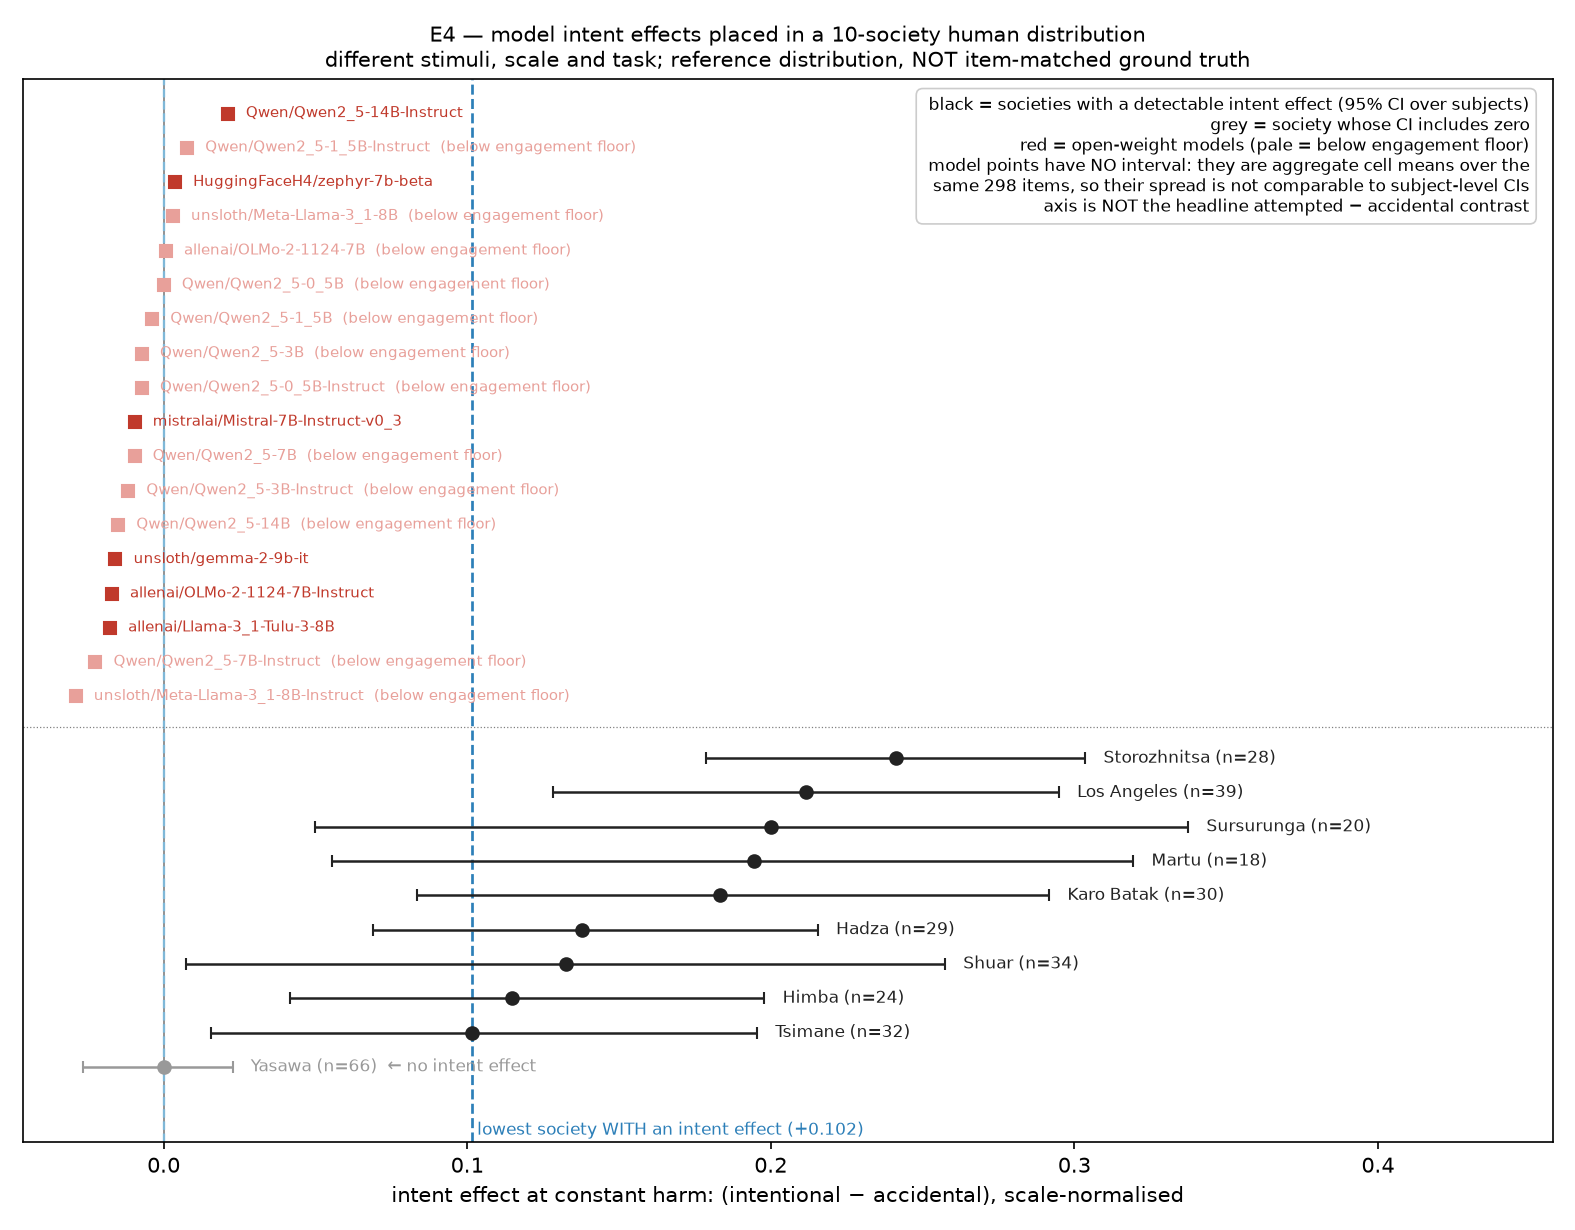
\includegraphics[width=\columnwidth]{figures/crosscultural_placement.png}
    \caption{Intentional-minus-accidental effect for ten societies (subject-level intervals) and open models (aggregate cell means). Stimuli, scales, and tasks differ.}
    \label{fig:culture}
\end{figure}

\subsection{Where the profile arises}
In three public post-training pipelines, base models were near zero and moved negative after supervised fine-tuning (SFT; \autoref{fig:stages}): SFT alone shifted OLMo-2 by $-0.588$, Tulu-3 by $-0.265$, and Zephyr by $-0.149$, accounting for 85.4\%, 65.4\%, and 27.0\% of each total shift; Zephyr's preference-optimization stage accounted for the remaining 73.0\%.
Across post-trained stages, $\outcomebeta/\intentbeta$ ranged from 3.0 to 7.7.
In 26 Pythia-1.4B and 20 OLMo-2-7B pretraining checkpoints, intent and outcome structure in hidden-state geometry developed smoothly, but no pretraining checkpoint gave gradeable ratings; the first gradeable OLMo point was SFT.
Consistent with post-training shaping the readout, a 20-model variance decomposition assigned the largest unique share of rating variance (8.6\%) to the condition $\times$ base/instruct interaction.
In two pairs (Qwen2.5-7B and Llama-3.1-8B), base-model ratings barely changed when the story was replaced by the agent's name alone (mean absolute change 0.06 versus 0.29 for instruct models; difference $+0.24$ [0.22, 0.25]).

\begin{figure}[t]
    \centering
    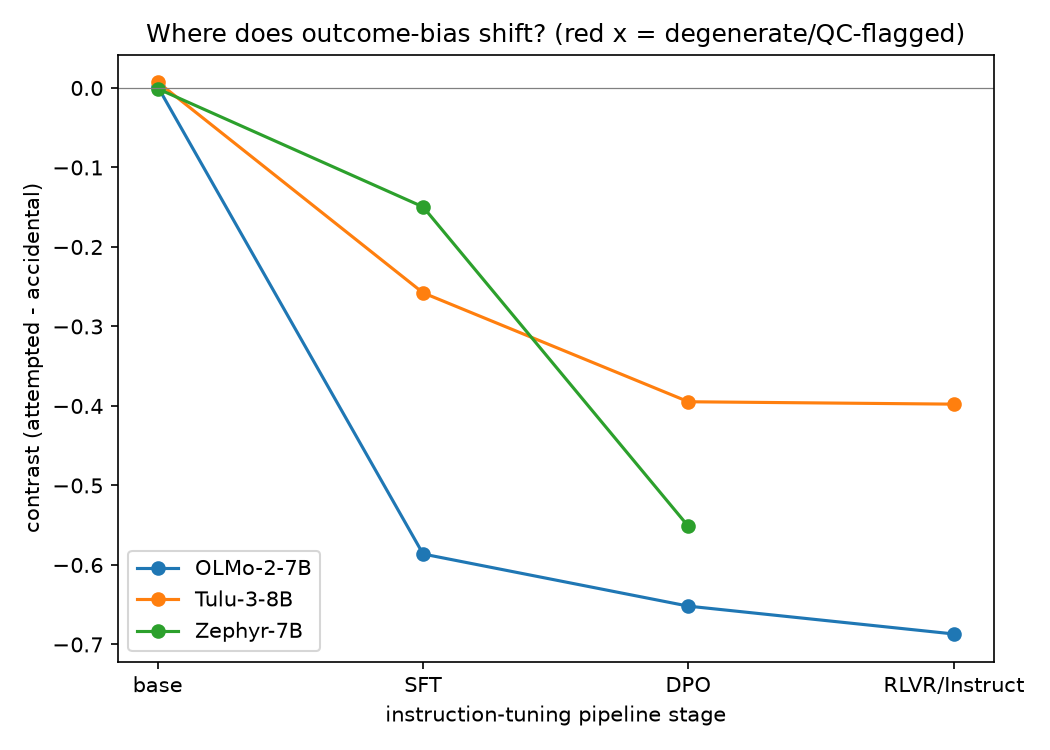
\includegraphics[width=0.92\columnwidth]{figures/checkpoint_dissection.png}
    \caption{Contrast across post-training stages in three public pipelines. SFT moves every family away from its near-zero base; the share attributable to later stages is recipe-dependent.}
    \label{fig:stages}
\end{figure}

\subsection{Converging internal evidence}
For eight open checkpoints, linear probes decoded intent at 0.90--0.98 at the end of the belief clause (span-matched lexical baseline 0.591).
Outcome was also decodable there (0.70--0.87 across 14 checkpoints, against a lexical baseline of 0.631), but a foreshadowing sentence is the only text before the belief-clause end that differs between outcome partners; deleting it reduced outcome decoding to chance (0.496--0.504 in all six models tested).
Early outcome decodability is therefore a readout of stated text, not prediction of an unstated outcome.
Yet item-level intent decodability did not predict intent-sensitive ratings (slope $+0.062$ [$-0.146$, $+0.270]$), and representational similarity did not track behavioral similarity across 28 model pairs ($r=+0.098$ [$-0.31$, $+0.46$]).
Adding the intent direction to hidden states changed the contrast by at most about 0.015, whereas an outcome direction changed it by 0.23--0.26 (\autoref{fig:steer}).
This was not because the manipulation failed internally: intent steering drove held-out intent decoding from about 0.89 to 0.50 while the rating contrast stayed nearly fixed.
Removing a linear outcome component made judgments more intent-sensitive in two of three models (contrast $+0.318$ and $+0.231$ with most of the four-cell spread retained); the third model's ratings collapsed instead, and specificity controls did not support an outcome-unique mechanism.

\begin{figure}[t]
    \centering
    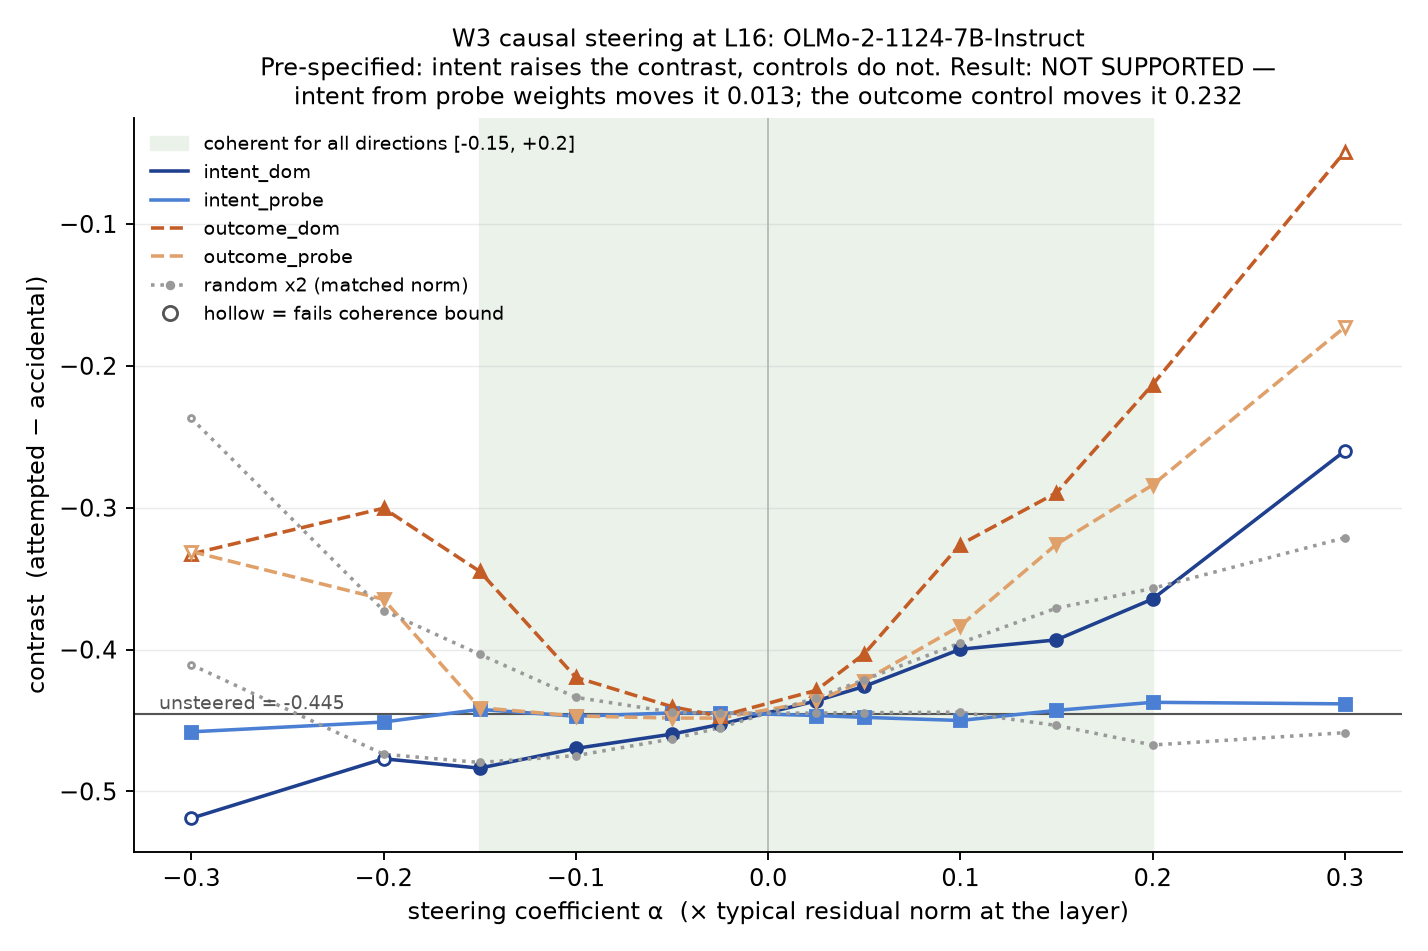
\includegraphics[width=\columnwidth]{figures/w3_steering_OLMo.png}
    \caption{Adding hidden-state directions in OLMo-2-7B-Instruct. The intent direction from probe weights (light blue squares) barely moves the contrast within the coherent range (shaded); outcome directions (orange) move it substantially; gray lines are matched random directions.}
    \label{fig:steer}
\end{figure}

\section{Discussion}

The central finding is a dissociation between \emph{stating} and \emph{using} mental-state information.
The same open instruct models that answer hard false-belief questions condemn accidents more than attempts, mention intent in most explanations while rating by outcome, and carry linearly decodable intent that does not control their ratings.
These results do not show that models lack all ToM-like computation, nor do they reduce to a binary of ``pattern matching'' versus ``reasoning.''
They show that explicit benchmark success is insufficient evidence of stable, human-reference use of intent in a downstream judgment.

Resemblance and mechanism also need to be kept apart.
Four closed models more closely matched the adult direction, but without internal access and item-matched human data, behavioral resemblance does not establish a human-like mechanism.
Conversely, outcome-weighted profiles are not categorically non-human: young children and some societies weight outcomes heavily \citep{cushman2013development,barrett2016societies}.
The developmental parallel is descriptive only; our checkpoint data suggest that pretraining yields structured intent and outcome representations while post-training determines how ratings express them, which is a different process from child development.

For cognitive science, the paradigm suggests a general recipe for evaluating machine ToM: report explicit inference, full factorial profiles of applied judgment, and robustness across prompts and training stages separately, and keep human comparisons descriptive unless the data are item-matched.

\textbf{Limitations.}
The open roster tops out at 14B parameters and half are Qwen2.5 models.
Human references come from different items and measures, and the reliability estimates cover model raters only: a scanner replication of the 2008 design lacks responses on 39.6\% of trials and a story-to-scenario mapping, so it cannot serve as an item-matched human anchor.
Reprinted scenarios reduce the effective sample to 53 groups.
Intent and outcome are expressed lexically, so representational analyses cannot fully separate meaning from wording.
Closed results are behavior-only and provisional.
Linear probes and interventions cannot rule out nonlinear or distributed intent use.

\section{Acknowledgments}
Initial submission: AI-use statement only, per CogSci policy.
Portions of this manuscript were drafted with an AI writing assistant from the authors' verified project results; the authors must describe this use in full and confirm all content before submission.

\printbibliography

\end{document}
